
\documentclass[12pt, a4paper, twoside]{book}
% TeX encoding = utf8
% TeX spellcheck = pl_PL 
\usepackage[OT4]{polski}
\usepackage[utf8]{inputenc} 
\usepackage{graphicx}

\author{Maciej Lotz }
\title{Robot IRp-6 w zadaniu śledzenia konturu}
\date{\today}



\begin{document}
	\sloppy
		
		
		\thispagestyle{empty}
		
		\begin{titlepage}
			\noindent
			\begin{flushright}
				\begin{tabular}[t]{r}
					\scriptsize Rok akademicki 2014/2015\\[5mm]
				\end{tabular}
			\end{flushright}
			\begin{center}
				\begin{tabular}[t]{c}
					\scriptsize POLITECHNIKA WARSZAWSKA\\
					\scriptsize WYDZIAŁ ELEKTRONIKI I~TECHNIK INFORMACYJNYCH\\
					\scriptsize INSTYTUT AUTOMATYKI I~INFORMATYKI STOSOWANEJ
				\end{tabular}
			\end{center}
			\vfill
			\begin{center}
				\resizebox{3.5cm}{!}
				{
					
\includegraphics{images/logo_politechnika.pdf}
				}
				\\[5mm]\textbf{PRACOWNIA DYPLOMOWA 1}\\[3mm] \textbf{SPRAWOZDANIE} \\[15mm]
				\large Maciej Lotz\\[10mm]
				\Large \textbf{Robot \mbox{\mbox{IRp-6}} w zadaniu śledzenia konturu}
			\end{center}
			
			\vspace{20mm}
			\begin{flushright}
				\begin{tabular}{l}
					Opiekun pracy:\\
					\large dr inż. Tomasz Winiarski
				\end{tabular}
			\end{flushright}
			\vfill
			\begin{tabular}{c}
				\scriptsize Ocena pracy: \dotfill\\[10mm]
				\scriptsize \makebox[55mm]{\dotfill}\\
				\scriptsize Data i~podpis Promotora\\
				
			\end{tabular}
		\end{titlepage} 	


\newpage
\tableofcontents

\chapter{Wymagania stawiane pracy}
	\section{Cel pracy dyplomowej}
	Celem pracy dyplomowej jest stworzenie i przetestowanie algorytmu realizującego śledzenie konturu obiektu z wykorzystaniem czujników siły oraz wspomaganie procesu za pomocą odczytów z kamery.
	\section{Wizja rozwiązania}
	Zadanie składa się z dwóch zagadnień:
		\subsection{Siłowe śledzenie konturu}
		Polega na wykryciu wektora siły działającego na końcówkę narzędzia. Na podstawie tego wektora można analitycznie wyznaczyć wektor prędkości, który ma być styczny do krawędzi i prostopadły do wektora siły. Teoretycznie umożliwi to poruszanie się po krawędzi z zachowaniem przyłożenia do niej zadanej siły.
		\subsection{Wspomaganie wizyjne}
		Powyższa metoda może być zawodna w przypadku gwałtownych zmian wektora siły, tzn. ostrych krawędzi konturu. W celu wyeliminowania zagrożenia wprowadzono wspomaganie wizyjne, które na podstawie odczytów z kamery, będzie w stanie wykryć takie gwałtowne zmiany i odpowiednio zareagować. Widzę dwie możliwe realizację:
			\subsubsection{Wspomaganie globalne}
			Robot sporządza mapę konturu i posiłkuje się nią w trakcie śledzenia krawędzi.
			\subsubsection{Wspomaganie lokalne}
			Robot śledzi kontur z kamerą skierowaną w kierunku wektora prędkości. W czasie rzeczywistym rozpoznaje załamania obiektu i jest w stanie odpowiednio szybko zareagować.
			\subsubsection{Nie wykluczam zastosowania hybrydy obu powyższych rozwiązań.}
\chapter{Wstęp teoretyczny}
	\section{Manipulator IRp-6}
	Manipulator IRp-6 to robot przemysłowy wykorzystywany w fabrykach do wykonywania czynności żmudnych lub niebezpiecznych. Na potrzeby laboratorium wzbogacony on został o końcówkę chwytną, kamerę oraz, w przypadku Tracka, mobilną platformę. 
	\section{Czujnik siły}
	W ostatnim przegubie robot IRp-6 ma zainstalowane czujniki siły, które są w stanie wykryć siły działające na końcówkę chwytną. Mechanizm ten pozwoli śledzić krawędź przy zachowaniu odpowiedniego nacisku.
	\section{ROS}
	ROS(Robot Operating System) to zespół bibliotek i narzędzi, które pozwalają na budowę oprogramowania dla robotów. Zawiera sterowniki realizujące operacje niskopoziomowe. Umożliwia również komunikację między wątkami i wizualizację robota w trójwymiarze.
	\section{IRPOS}
	Stworzony przez Zespół Programowania Robotów i Systemów Rozpoznających IRPOS to biblioteka wysokopoziomowych funkcji służących do sterowania robotem. Wykorzystanie i wprowadzanie modyfikacji jest względnie łatwe.
\chapter{Opis tego co zrobiono dotychczas}
	\section{Konfiguracja środowiska}
	W celu przygotowania się do pracy w laboratorium wykonano następujące czynności:
		\begin{itemize}
			\item Zainstalowano ROS na stacji roboczej.
			\item Zainstalowano i skonfigurowano Eclipse.
			\item Założono nowe repozytorium na Githubie.
		\end{itemize}		
	\section{Opanowanie podstaw języka Python}
	Skrypty IRPOSa są napisane w języku Python, dlatego konieczne było opanowanie tego języka. Ponadto Zapoznałem się z pakietem naukowym NumPy. Pakiet NumPy umożliwia między innymi prowadzenie obliczeń na macierzach, co będzie potrzebne do wykonania głównego zadania.
	\section{Wykonanie specjalistycznego narzędzia do śledzenia krawędzi}
	W celu realizacji zadania śledzenia konturu konieczne było wykorzystanie specjalnego narzędzia. Zostało ono zaprojektowane tak, aby robot mógł je chwycić i utrzymać pewny chwyt podczas śledzenia krawędzi pomimo dużych sił występujących w miejscu kontaktu z obiektem. Na końcu narzędzia zamontowano łożysko w celu wyeliminowania tarcia ze śledzonym konturem.
	
	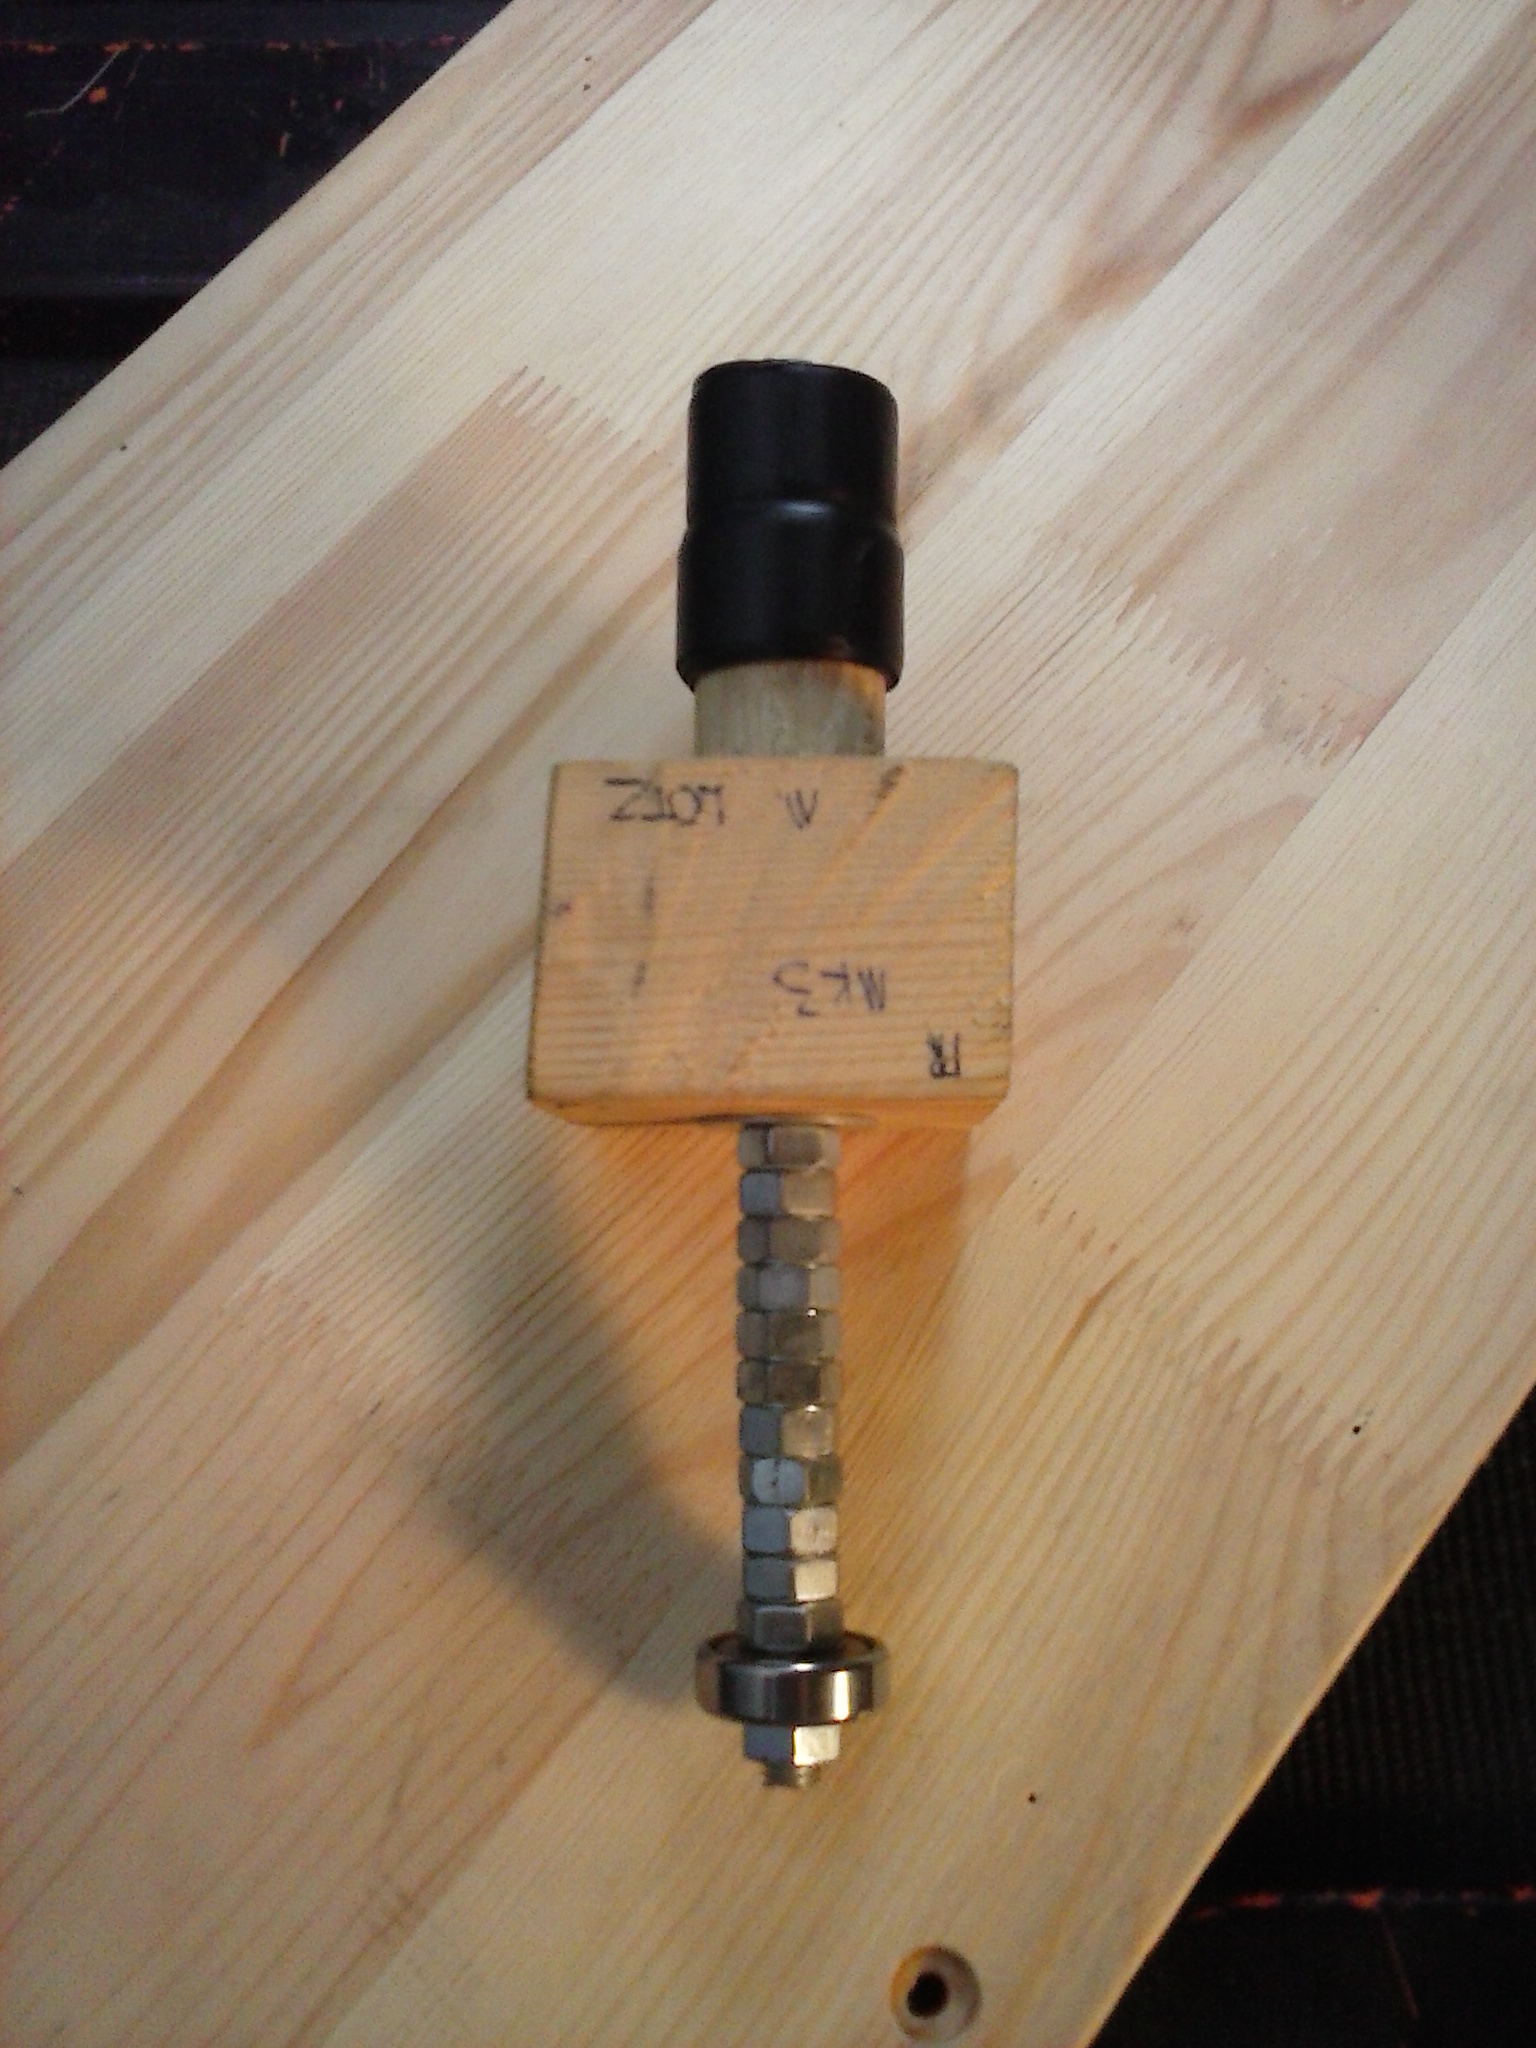
\includegraphics[width=7.5cm,height=10cm]{images/MK3.jpg}
	
	Rys. 1 Narzędzie do śledzenia krawędzi
	
	\section{Wykonanie ćwiczeń pobocznych}
		\subsection{Rysowanie kwadratu w powietrzu}
		Ćwiczenie umożliwiło dobre zapoznanie się z systemem IRPOS oraz oswojenie z robotem.
		\subsection{Znajdowanie środka okręgu na podstawie trzech punktów}
		Przebieg algorytmu:
			\begin{enumerate}
			\item Ustawić ramię w pozycji roboczej.
			\item Obniżać końcówkę do kontaktu z podłożem.
			\item Przesuwać narzędzie w osi X do kontaktu z obręczą. Zapisać pozycję bezwzględną końcówki.
			\item Przesuwać narzędzie w osi X w przeciwnym kierunku do znalezienia drugiego kontaktu. Zapisać pozycję bezwzględną końcówki.
			\item Przesuwać w osi Y do znalezienia trzeciego kontaktu. Zapisać pozycję bezwzględną końcówki.
			\item Na podstawie trzech punktów wyliczyć analitycznie środek obręczy.
			\item Przesunąć końcówkę do środka obręczy. 
			\end{enumerate}
		Celem ćwiczenia była nauka obsługi czujnika siły oraz korzystania z pakietu NumPy dla macierzy.
	\section{Zrealizowanie śledzenia konturu prostego}
		Ćwiczenie polegało na śledzeniu konturu będącego prostą. Stanowiło ono pierwsze przymiarki do realizacji głównego zadania.
			
\chapter{Plany na kolejny semestr}
	\section{Zrealizowanie śledzenia konturu}
	Pierwszym zadaniem na przyszły semestr będzie stworzenie algorytmu śledzenia skomplikowanych krawędzi.
	\section{Opanowanie OpenCV i DisCODe}
	Konieczne będzie opanowanie bibliotek przetwarzania obrazu. Zamierzam wykorzystać odczyty z kamery do wspomagania śledzenia konturu.
\end{document}